\section{Reduced Order Surrogate}
\label{sec:ros}

In this section, we focus our attention on constructing a surrogate that captures the dependence of
uncertainty in NEMD predictions for the bulk thermal conductivity ($\kappa$) on input variability
in the SW potential parameters. The surrogate is a powerful tool that greatly minimizes
the computational
effort required for forward propagation of the uncertainty from input parameters to the observable,
Sobol sensitivity analysis, and Bayesian calibration of the uncertain model parameters. Once again,
we use polynomial chaos (used to construct response surfaces for discrepancy in
Section~\ref{sec:response}) to construct the surrogate of the following functional form:

\be
\kappa  = \sum\limits_{\bm{s}\in\mathcal{A}} c_{\bm{s}}(T)\Psi_{\bm{s}}(\bm{\xi})
\ee

As discussed earlier in Section~\ref{sec:response}, several strategies are available to
estimate the PC coefficients, $c_{\bm{s}}$. However, since the polynomial basis functions
($\Psi_{\bm{s}}(\bm{\xi}$)) are
relatively high dimensional, we use a computationally efficient approach proposed by
Blatman and Sudret to construct a PCE with sparse basis($\mathcal{A}$) using the LAR
algorithm~\cite{Blatman:2011}. Furthermore, since the NEMD simulations are compute-intensive,
estimating the PC coefficients in the 7D parameter space would still require large amount of
computational resources. Hence, we explore the possibility of reducing the dimensionality of
the surrogate. For this purpose, we 
exploit our observations in Figure~\ref{fig:ub} where a significant
jump in $\hat{\mathcal{C}_i\mu_i}$ estimate is seen from $A$ to $B$ and thereby construct the 
PC surrogate in a 5D parameter space by fixing $B$ and $p$ at their nominal values. In the above
equation, $\bm{\xi}:~\{\xi_1(A),\xi_2(q),\xi_3(\alpha),\xi_4(\lambda),\xi_5(\gamma)\}$ is a set
of five canonical random variables, $\xi_i$ distributed uniformly in the interval [-1,1].
Prior intervals for the uncertain SW parameters are considered to be
$\pm~10\%$ of their respective nominal estimates except for $q$ in which case it is [0,0.1]. In
Figure~\ref{fig:loo}, we plot the leave-one-out cross-validation error 
($\epsilon_{\tiny{\mbox{LOO}}}$)~\cite{Blatman:2010}, defined
below in Eq.~\ref{eq:loo}, against the number of model realizations used to construct the 5D
PC surrogate. UQLab~\cite{Marelli:2014} was used for estimating $\epsilon_{\tiny{\mbox{LOO}}}$ and constructing
the surrogate. 

\be
\epsilon_{\tiny{\mbox{LOO}}} = \frac{\sum\limits_{i=1}^{N}\left(\mathcal{M}(\bm{x}^{(i)}) - 
\mathcal{M}^{PCE\setminus i}(\bm{x}^{(i)})\right)^{2}}{\sum\limits_{i=1}^{N}
\left(\mathcal{M}(\bm{x}^{(i)}) - \hat{\mu}_Y\right)^2}
\label{eq:loo}
\ee 

\noindent where $N$ denotes the number of realizations, $\mathcal{M}(\bm{x}^{(i)})$ is the
model realization and $\mathcal{M}^{PCE\setminus i}(\bm{x}^{(i)})$ is the corresponding PCE estimate
at $\bm{x}^{(i)}$. Note that the PCE is constructed using all points except $\bm{x}^{(i)}$.
The quantity, $\hat{\mu}_Y$ = $\frac{1}{N}\sum\limits_{i=1}^{N}\mathcal{M}(\bm{x}^{(i)})$
is the sample mean of the realizations.

\begin{figure}[htbp]
 \begin{center}
  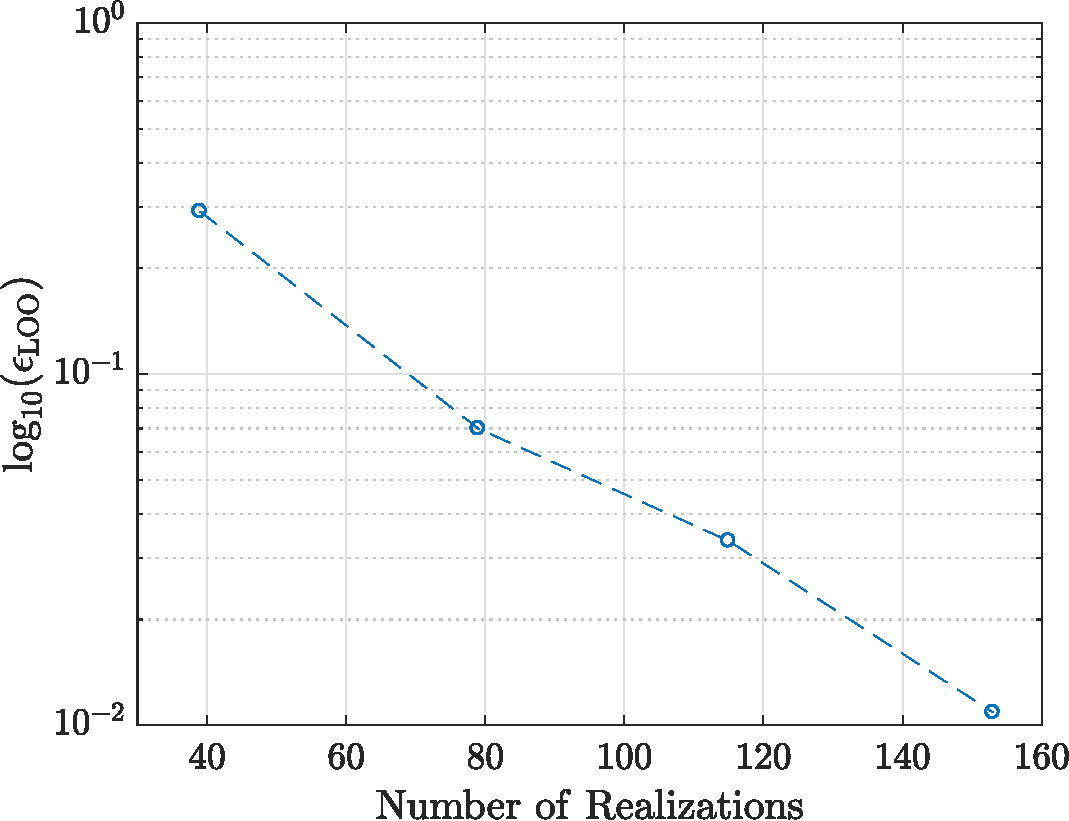
\includegraphics[width=0.70\textwidth]{./Figures/PCE5D_eloo}
\caption{A convergence study for the 5D PCE wherein the leave-one-out
error, $\epsilon_{\tiny{\mbox{LOO}}}$ is plotted against the number of
realizations or NEMD runs used to estimate the PC coefficients.}
\label{fig:loo}
\end{center}
\end{figure}
 
It is found that in order for the PCE to converge to an accuracy of~$\mathcal{O}(10^{-2})$
with respect to $\epsilon_{\tiny{\mbox{LOO}}}$, we require approximately 160 NEMD runs. In the
following section, we focus on verifying the accuracy of the 5D PCE against the set of available
NEMD predictions in the original 7D parameter space. 

\subsection{PC Surrogate Verification}

The accuracy of the 5D PC surrogate is verified using two different strategies. The first strategy involves
computing the relative L-2 norm of the difference between the available NEMD predictions (used earlier
to estimate DGSM in Section~\ref{sec:sense}) and estimates using the 5D surrogate as follows:

\be
\epsilon_{\mbox{\tiny{L-2}}} = 
\frac{\left[\sum\limits_{i=1}^{N=25}\left(\mathcal{M}(\bm{\theta}_{\mbox{\tiny{7D}}}^{(i)}) - 
\mathcal{M}^{PCE}(\bm{\theta}_{\mbox{\tiny{5D}}}^{(i)})\right)^{2}\right]^{\frac{1}{2}}}{\left[\sum_{i=1}^{N}
\left(\mathcal{M}(\bm{\theta}_{\mbox{\tiny{7D}}}^{(i)})\right)^2\right]^{\frac{1}{2}}} \approx 6.88\times 10^{-2}
\ee
 
\noindent where $\mathcal{M}(\bm{\theta}_{\mbox{\tiny{7D}}}^{(i)})$ is the NEMD prediction in the original 7D
parameter space, and $\mathcal{M}^{PCE}(\bm{\theta}_{\mbox{\tiny{5D}}}^{(i)})$ is the corresponding 
estimate using the reduced order surrogate (5D). 
Since $\epsilon_{\mbox{\tiny{L-2}}}$ is found to be $\mathcal{O}(10^{-2})$, the 5D surrogate can be considered as
reasonably accurate from the perspective of relative L-2 error norm. 

\begin{figure}[htbp]
 \begin{center}
  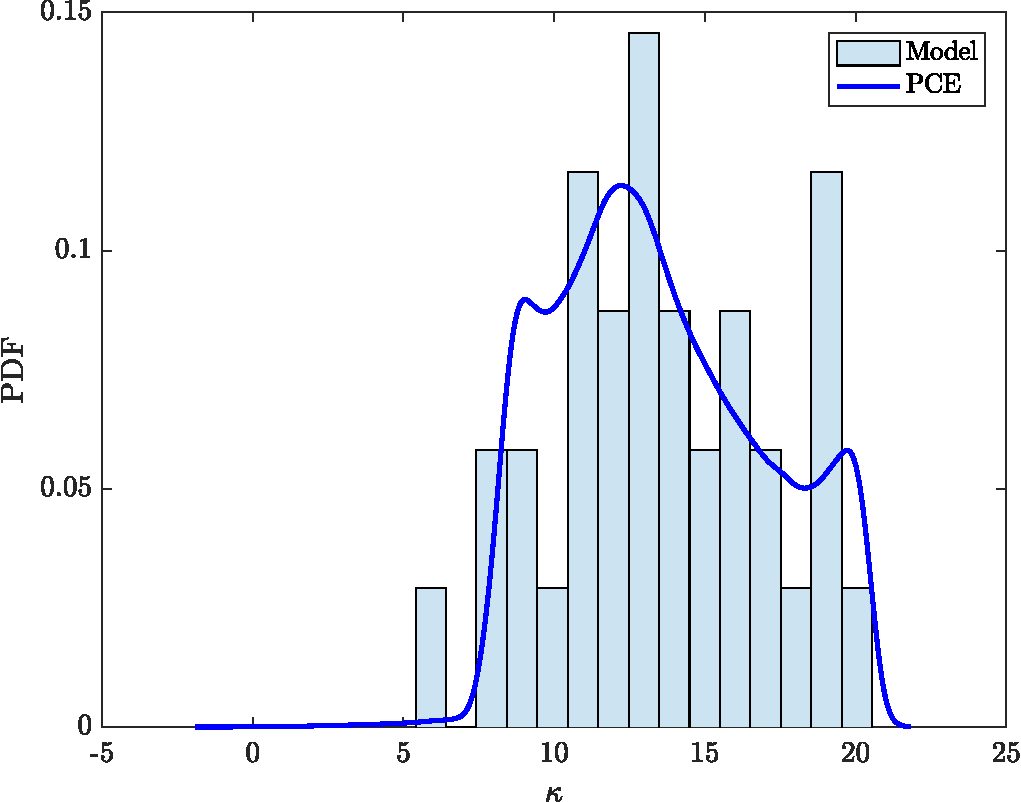
\includegraphics[width=0.70\textwidth]{./Figures/PCE5D_kde}
\caption{Comparison of bulk thermal conductivity ($\kappa$) distribution of Si based on a histogram plot
using NEMD predictions (Model) at 25 points in the 7D parameter space and a probability distribution obtained 
using kernel density estimation of  reduced order surrogate estimates of $\kappa$ for 10$^6$ samples in the 5D
parameter space.}
\label{fig:verify}
\end{center}
\end{figure}

In the second strategy, we compare NEMD
predictions and estimates from the 5D surrogate in a probabilistic sense. As shown in Figure~\ref{fig:verify}, a 
histogram plot based on the available set of NEMD predictions for bulk thermal conductivity in the 7D parameter 
space is compared with its probability distribution, obtained using the reduced order surrogate and
10$^6$ samples in the 5D parameter space described by the SW potential parameters:~$\{A,q,\alpha,\lambda,\gamma\}$. It is observed that the probability distribution (PDF) based on estimates from the reduced order surrogate compares
favorably with the histogram. Specifically, the corresponding mode values for $\kappa$ from the two plots are
in close agreement, and the PDF reasonably captures the peaks as well as the spread in
the bulk thermal conductivity distribution as observed in the histogram. 
Hence, the reduced order surrogate is verified for accuracy in both cases. 
\bigskip

As mentioned earlier, a PC surrogate can be used to estimate Sobol global sensitivity indices in a 
straightforward manner~\cite{Sudret:2008}. Sobol first order and total effect sensitivity indices as estimated
using the reduced order surrogate and $10^{6}$ samples in the 5D parameter space are plotted using bar-graphs in
Figure~\ref{fig:gsa}. 

\begin{figure}[htbp]
 \begin{center}
  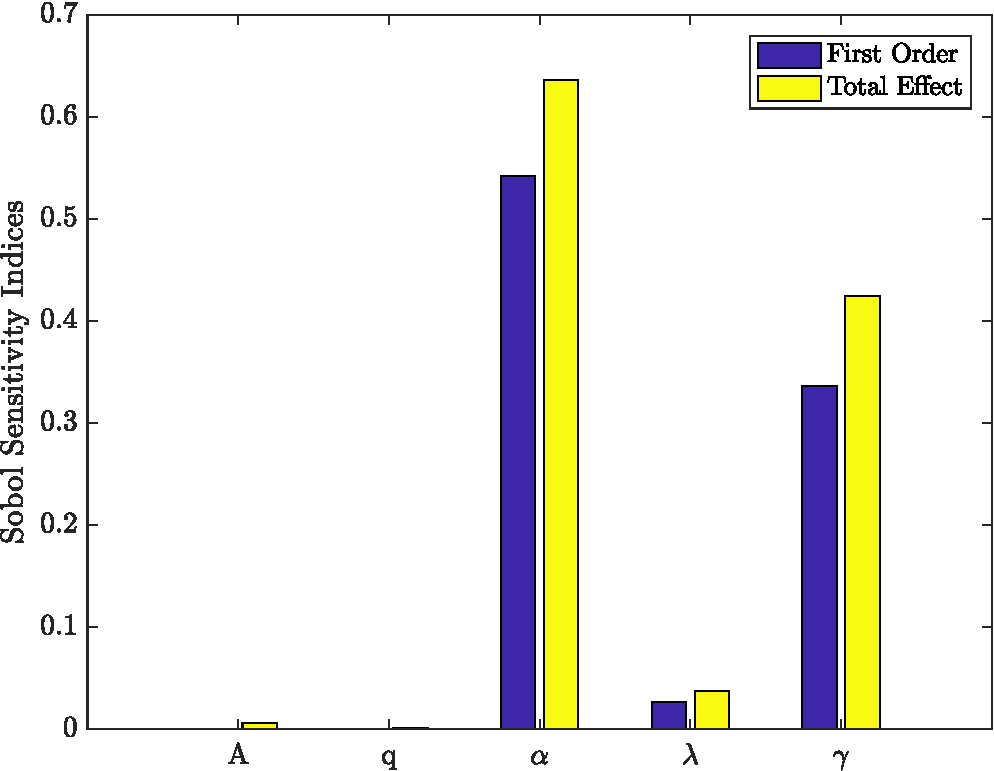
\includegraphics[width=0.70\textwidth]{./Figures/PCE5D_gsa}
\caption{Sobol first-order and total effect sensitivity indices as obtained using the reduced order PC
surrogate and 10$^{6}$ samples in the 5D parameter space. }
\label{fig:gsa}
\end{center}
\end{figure}

It is found that $\kappa$ is predominantly sensitive towards the choice of $\alpha$ and
$\gamma$. This observation is consistent with our initial findings based on DGSM using 25 samples in the 7D
parameter space. However, the DGSM estimate for $\gamma$ was found to be the highest in that case. 
While sensitivity towards $A$, $q$, and $\lambda$ is observed to be comparatively less in both cases, Sobol
indices for the three parameters are estimated to be smaller by an order of magnitude compared to those
for $\alpha$ and $\gamma$. Large quantitative disagreement in parametric sensitivity between DGSM and the 
Sobol indices is however not unexpected essentially because the two metrics differ by construction.
The former is based
on an expectation of partial derivatives while the later is based on variance. Nevertheless, significant qualitative
agreement pertaining to parameter importance in the two approaches is quite encouraging. 
Moreover, verification of the reduced order
surrogate for accuracy increases our confidence in implementing DGSM to ascertain relative importance of the
SW potential parameters and hence perform uncertainty analysis for the present application with minimal
computational effort. 


























